\subsubsection{PVT}
Position from the pseudoranges and the decoded ephemeris, compared with the surveyed antenna position (-23.209433$^\circ$, -45.874875$^\circ$, 596.42~m).

\begin{figure}[H]
  \centering
  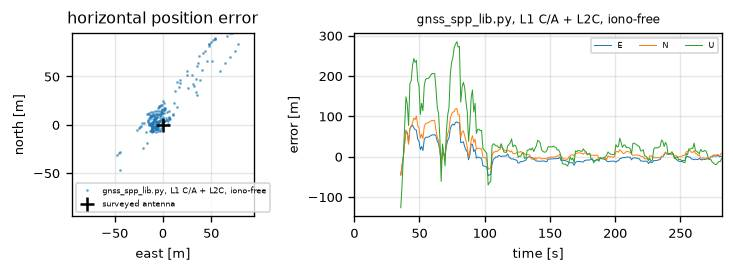
\includegraphics[width=1.0\linewidth]{gnss_sdr/x310_20261023T193310Z/pvt_spp.jpg}
  \caption{PVT: position error of the gnss\_spp\_lib.py solution with respect to the surveyed antenna position: computed from GNSS-SDR's observables and decoded GPS ephemeris, removing the ionospheric delay with the second band (pseudoranges carrier-smoothed over 100~s).}
\end{figure}

\begin{figure}[H]
  \centering
  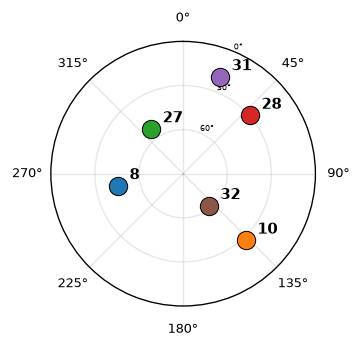
\includegraphics[width=0.45\linewidth]{gnss_sdr/x310_20261023T193310Z/skyplot.jpg}
  \caption{PVT: sky plot of the GPS satellites in the gnss\_spp\_lib.py dual-frequency solution (azimuth, elevation) during the recording.}
\end{figure}

\begin{table}[H]
  \centering
  \footnotesize
  \resizebox{\ifdim\width>\linewidth\linewidth\else\width\fi}{!}{%
  \begin{tabular}{l>{\centering\arraybackslash}p{4.2cm}}
    \hline
    \textbf{Solution} & \textbf{gnss\_spp\_lib.py, L1 C/A + L2C, iono-free} \\
    \hline
    Solutions & 247 \\
    Run with fix [\%] & 88 \\
    Mean E / N / U [m] & 3.5 / 16.2 / 42.4 \\
    Std E / N / U [m] & 25.3 / 30.2 / 73.3 \\
    RMS 2-D [m] & 42.7 \\
    RMS 3-D [m] & 94.9 \\
    95\% horiz. [m] & 105.7 \\
    \hline
  \end{tabular}}
  \caption{PVT: position error statistics with respect to the surveyed antenna (mean = accuracy, std = precision; \% of the run's seconds with a position; gnss\_spp\_lib.py computes one per second).}
\end{table}

